\documentclass[11pt,a4paper]{article}
\usepackage[final]{acl}
\usepackage{times}
\usepackage{latexsym}
\renewcommand{\UrlFont}{\ttfamily\small}

\usepackage{microtype}
\usepackage{graphicx}
\usepackage{booktabs}
\usepackage{multirow}
\usepackage{subcaption}
\usepackage{amsmath}

\newcommand\BibTeX{B\textsc{ib}\TeX}

\title{Mining Political Framing and Moral Values from Spanish Parliamentary Transcripts: A Zero-Shot LLM and Distillation Pipeline}

\author{
  Andrés Malón \& Roberto Aldanondo \\
  Natural Language Processing Final Project \\
  MSc in Machine Learning at UPNA
}

\date{}

\begin{document}
\maketitle
\begin{abstract}
This report details the methodology and evaluation of a robust natural language processing pipeline designed to mine political framing and moral values from the ParlaMint-ES corpus of Spanish parliamentary transcripts. The core difficulty of identifying latent argumentative frames in unstructured parliamentary debate is addressed through a multi-phase taxonomy. We highlight a novel approach utilizing a heavyweight large language model (Qwen 2.5 72B Instruct) for zero-shot argument extraction and annotation. To overcome the computational constraints of deploying a 72B-parameter model for large-scale production, we distill this extracted knowledge into a highly efficient RoBERTa-base classifier, yielding rapid and scalable inference. 
\end{abstract}

\section{Introduction}
Argument mining in political discourse provides crucial insights into how politicians frame policies and appeal to the moral values of the electorate. Extracting and classifying these arguments from raw parliamentary transcripts, however, remains profoundly challenging due to the unstructured, colloquial, and often implicit nature of political rhetoric. We present an end-to-end NLP pipeline addressing this problem by analyzing the ParlaMint-ES dataset.

Our methodology leverages a multi-phase annotation scheme, transitioning from basic premise-stance-conclusion extraction to the identification of the 20 basic human values theorized by Schwartz (Touché23 ValueEval format), and finally to specialized Spanish Political Frames. The primary novelty of our framework is the reliance on a zero-shot heavyweight LLM—the Qwen 2.5 72B Instruct model—for initial high-quality annotation. This process generates a robust, labeled dataset. Recognizing the immense computational overhead and VRAM requirements of the 72B model, we subsequently employ knowledge distillation, fine-tuning an efficient Spanish RoBERTa-base model capable of rapid production inference on consumer-grade hardware.

\section{Related Work}
Our approach intersects with three key areas of natural language processing: argument mining, moral value identification, and ideological framing.

\textbf{Argument Mining (AM):} AM seeks to identify argumentative structures within unstructured text, such as premises, stances, and conclusions. Prior works have applied AM to various domains, though adapting it to the highly contextual nature of parliamentary debates continues to evolve. 

\textbf{Theory of Basic Human Values:} The Schwartz theory identifies universally recognized human values (e.g., universalism, security, power). In NLP, initiatives like the Touché23 ValueEval shared task have formalized the classification of text into these human values, providing a robust taxonomy for evaluating latent moral appeals in political discourse.

\textbf{Ideological and Political Framing:} Framing in political science refers to the specific angles or lenses (e.g., economic stability, social justice) through which political actors present issues. Detecting explicit and implicit frames is crucial for understanding polarization and ideological shifts within parliaments.

\section{Methodology}
Our architecture is organized into an extraction and cleaning pipeline, taxonomy phase structuring, feature engineering, and robust model training.

\subsection{Phase Taxonomies}
The pipeline implements an escalating taxonomy across three phases:
\begin{itemize}
    \item \textbf{Phase 1 (Unlabeled arguments):} Focused purely on extracting robust argumentation components (conclusion, stance, and literally quoted premise).
    \item \textbf{Phase 2 (Schwartz Values):} Each argument is mapped to the standard 20 Schwartz Basic Human Values taxonomy.
    \item \textbf{Phase 3 (Political Frames):} Arguments are classified into 10 definitive Spanish political frames, ensuring annotation strictly requires explicit invocation by the politician rather than assumed framing.
\end{itemize}

\subsection{Data Extraction and Cleaning}
The Qwen 2.5 72B Instruct model processed the raw transcripts sequentially. While the model excels at zero-shot reasoning, its output occasionally suffered from JSON structure hallucinations and dropped metadata (e.g., emitting keys like ``speaker'' instead of the expected ``Speaker''). We implemented aggressive regex parsing and metadata recovery protocols to salvage thousands of otherwise orphaned arguments, minimizing instances relegated to the ``Desconocido'' (Unknown) tag.

\subsection{Feature Engineering and Training}
Following text preprocessing, target tags were encoded using a MultiLabelBinarizer, forming the basis for stratified data splits. We constructed a custom \texttt{BalancedMultiLabelTrainer} using HuggingFace's Trainer API to mitigate severe class imbalances inherent in political framing taxonomies. The trainer leverages dynamic positive weighting with a \texttt{BCEWithLogitsLoss} function.

Our student model, \texttt{roberta-base-spanish}, was trained utilizing aggressive hardware optimizations compatible with Ada/Ampere architectures, including TF32 (TensorFloat-32) and BFloat16 precision, reducing VRAM pressure and accelerating matrix multiplications. Hyperparameter optimization was managed via Optuna across multi-label loss optimization.

\section{Experiments \& Results}
The final model was rigorously evaluated on a held-out test split, ensuring unbiased performance metrics, before undergoing a final production retraining phase incorporating all available data splits (Train + Val + Test).

\subsection{Quantitative Metrics}
The distilled RoBERTa classifier achieved the following performance on the hold-out test set:
\begin{itemize}
    \item \textbf{Macro-F1 Score:} 0.4981
    \item \textbf{Macro-Precision:} 0.5210
    \item \textbf{Macro-Recall:} 0.4771
\end{itemize}

\subsection{Individual Rhetorical Profiles}
To map ideological signatures, we generated Political Frame Radar charts based on the inference engine's classifications for selected political leaders.

\begin{figure}[htbp]
    \centering
    \begin{subfigure}[b]{0.45\linewidth}
        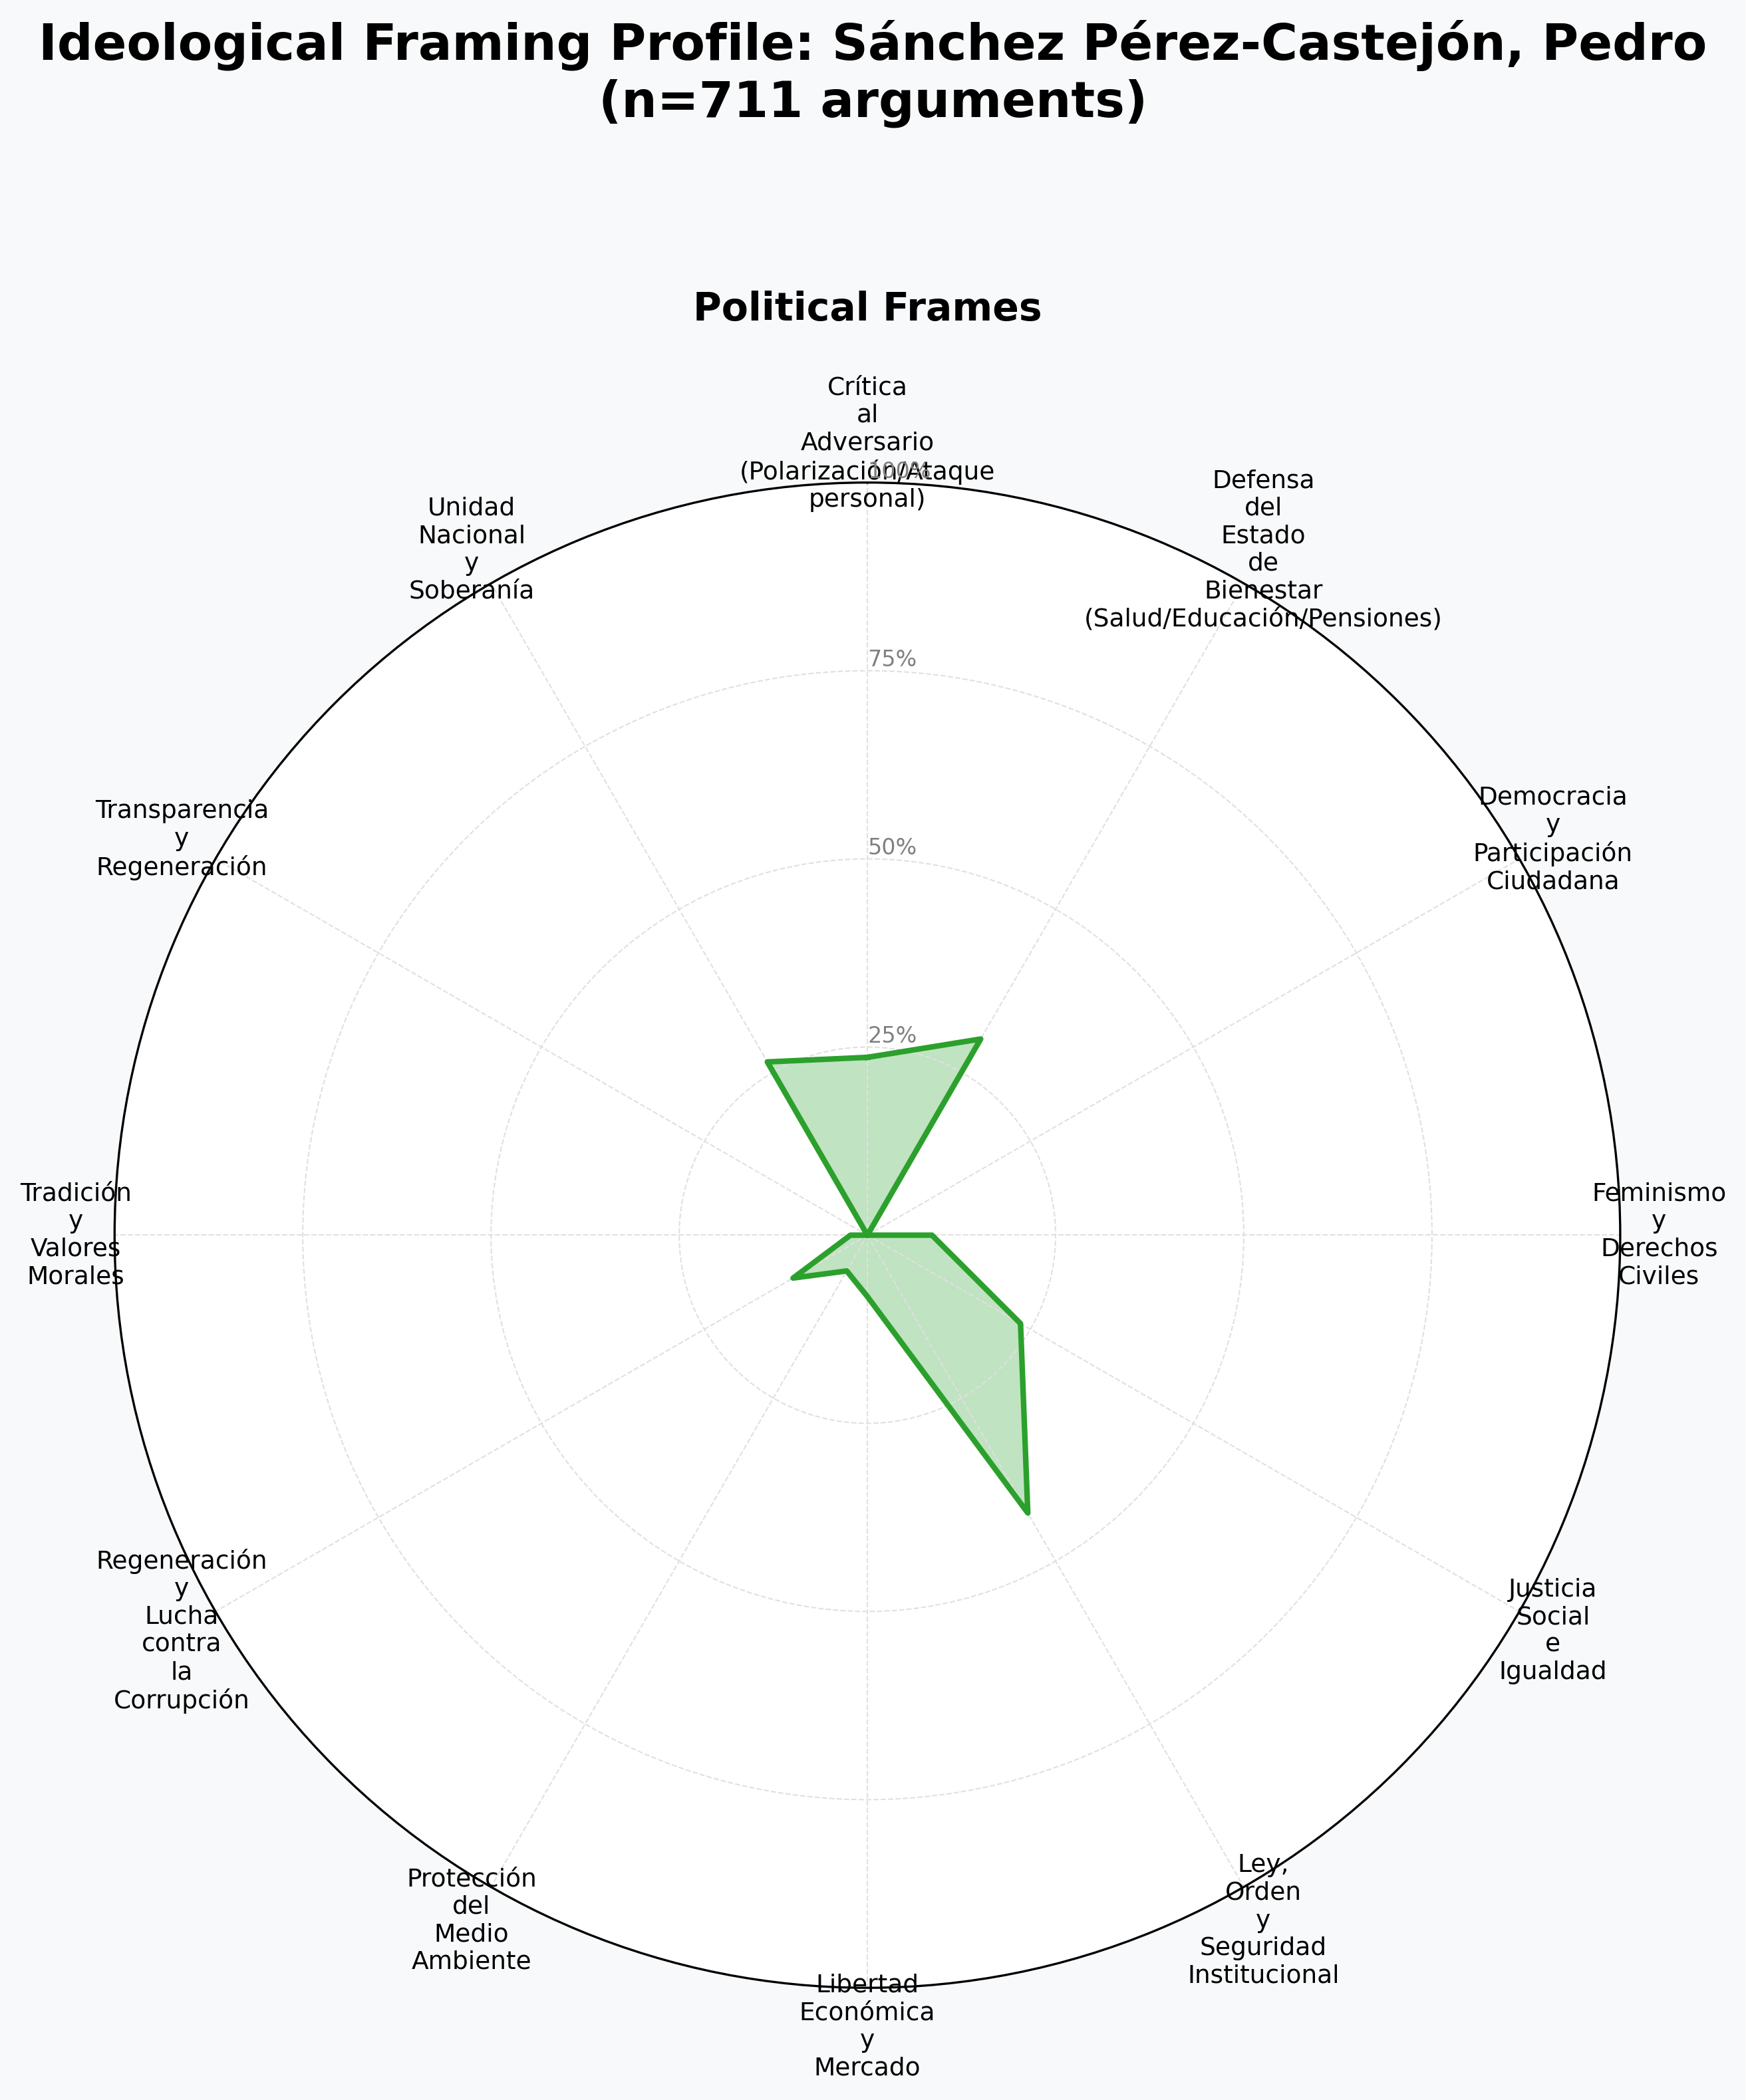
\includegraphics[width=\linewidth]{reports/figures/sánchez_pérez_castejón_pedro_phase_12_radar.png}
        \caption{Pedro Sánchez}
    \end{subfigure}
    \hfill
    \begin{subfigure}[b]{0.45\linewidth}
        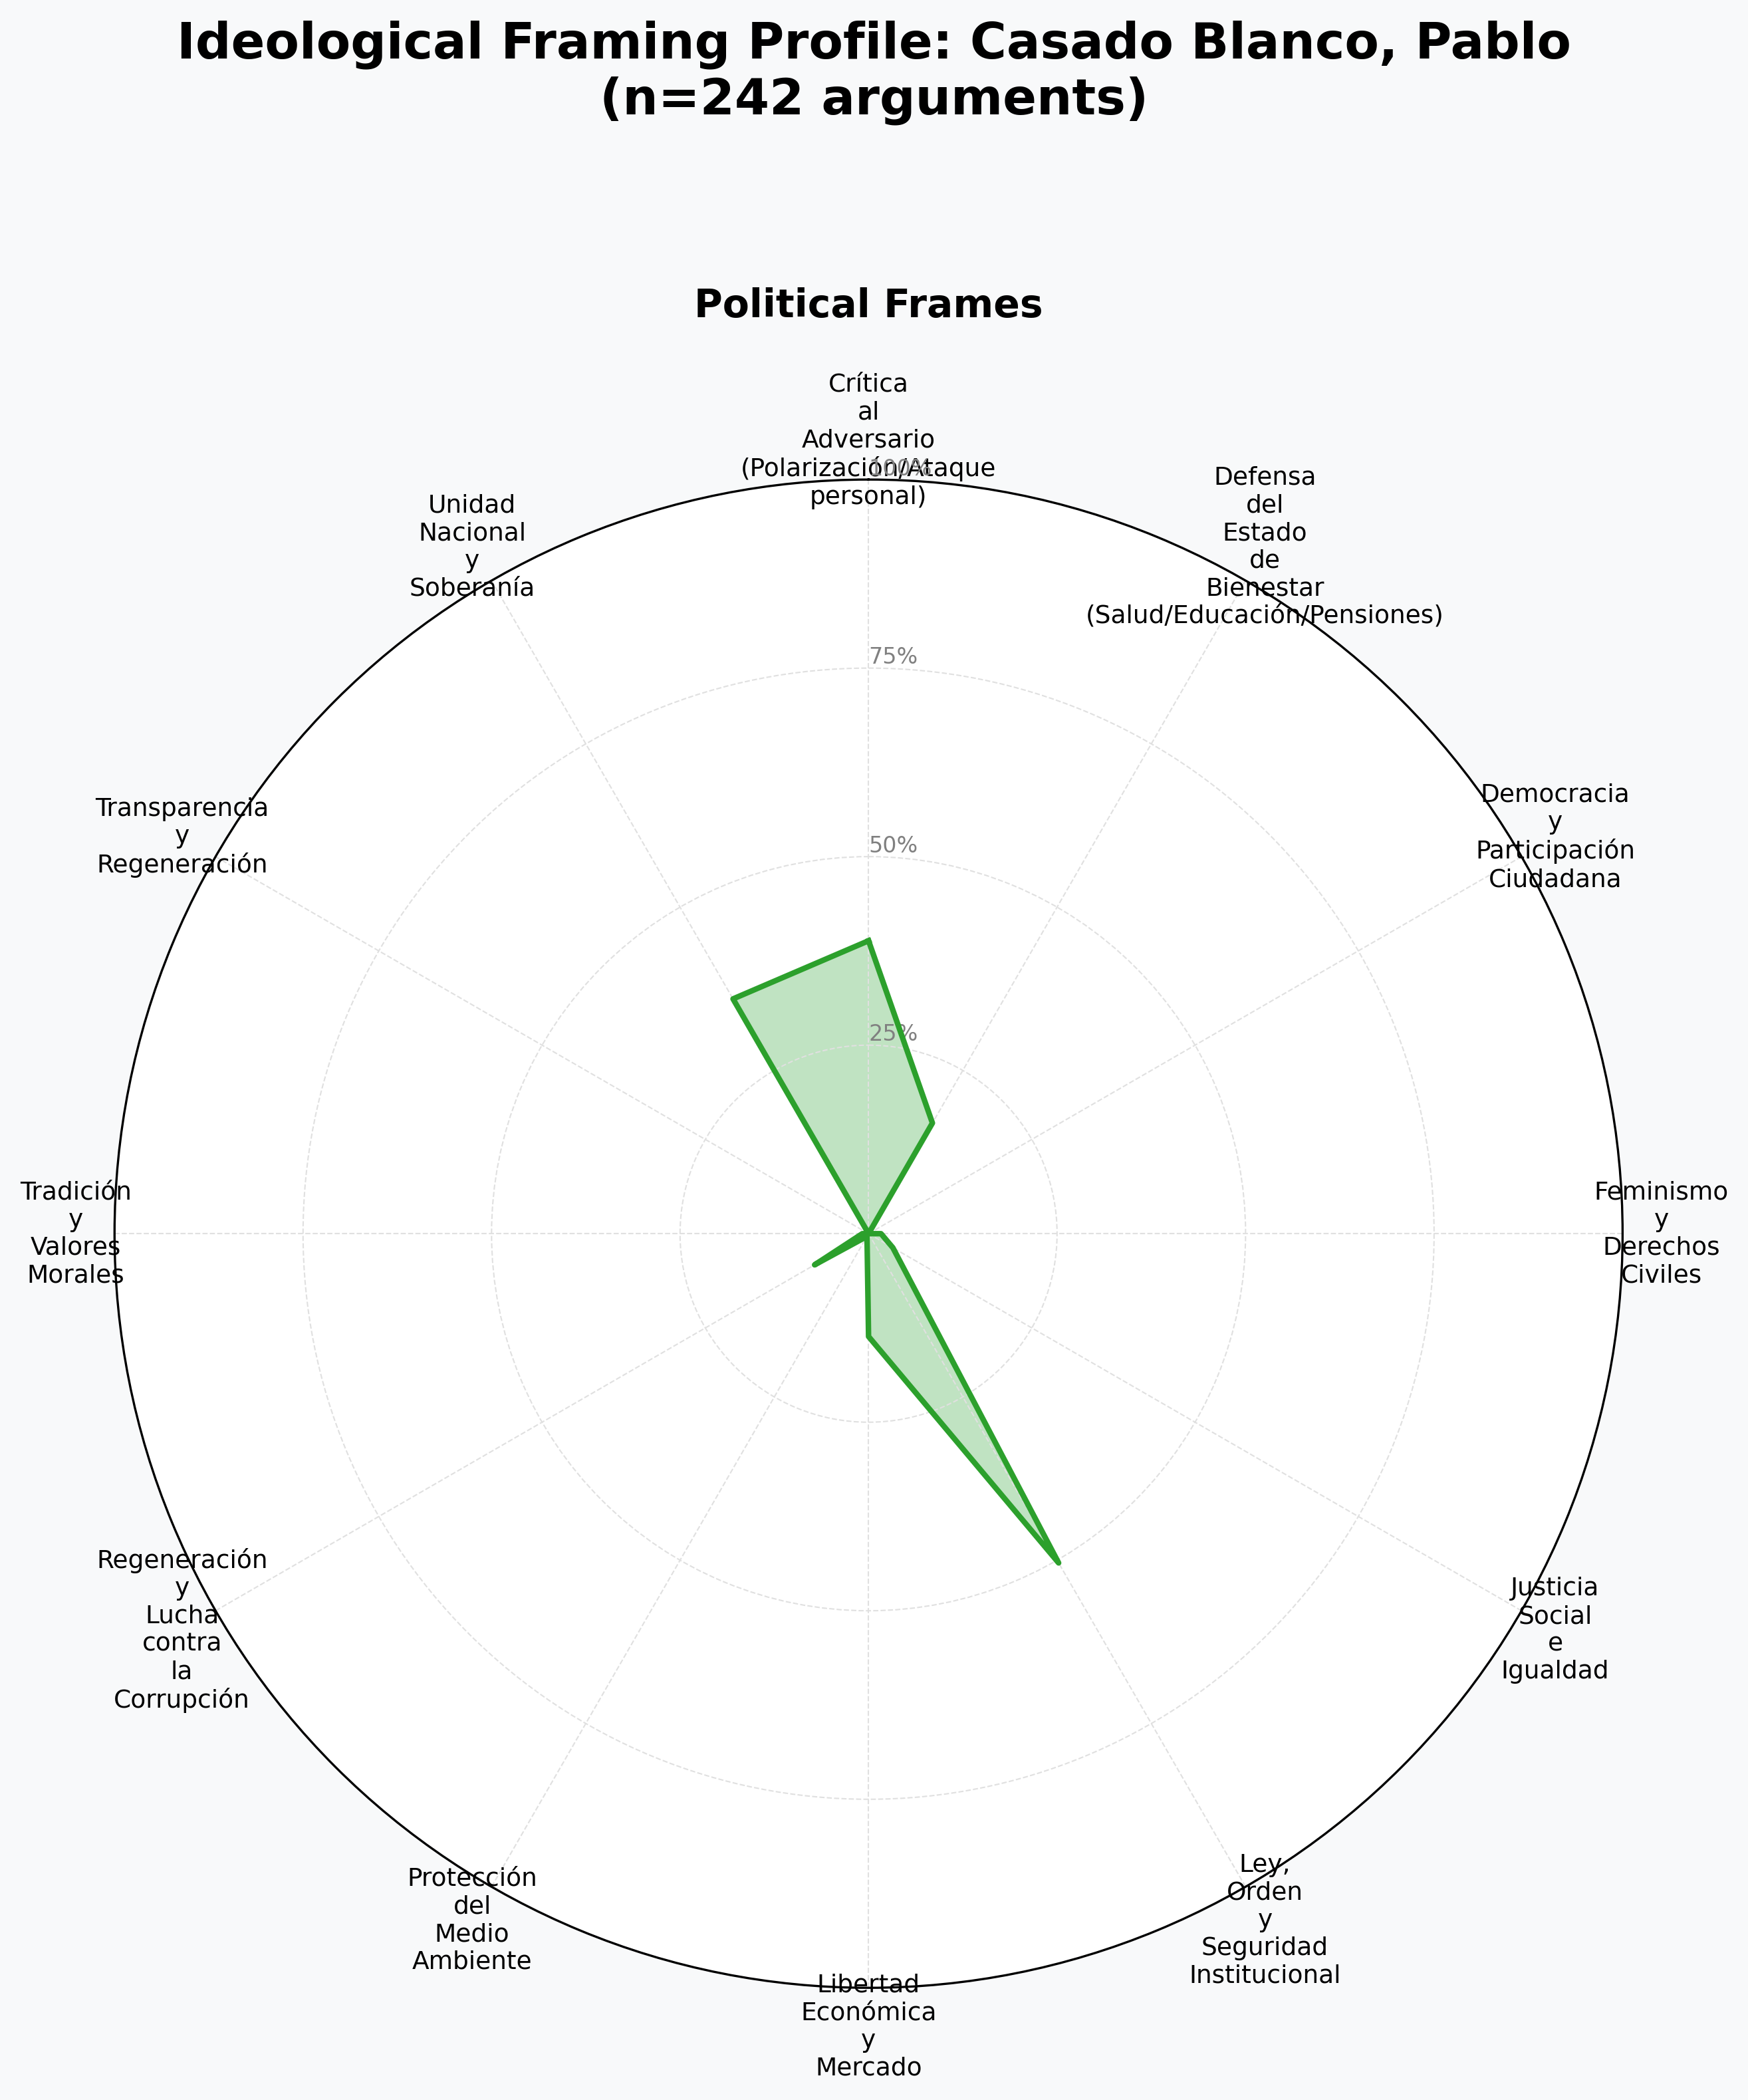
\includegraphics[width=\linewidth]{reports/figures/casado_blanco_pablo_phase_12_radar.png}
        \caption{Pablo Casado}
    \end{subfigure}
    \\
    \begin{subfigure}[b]{0.45\linewidth}
        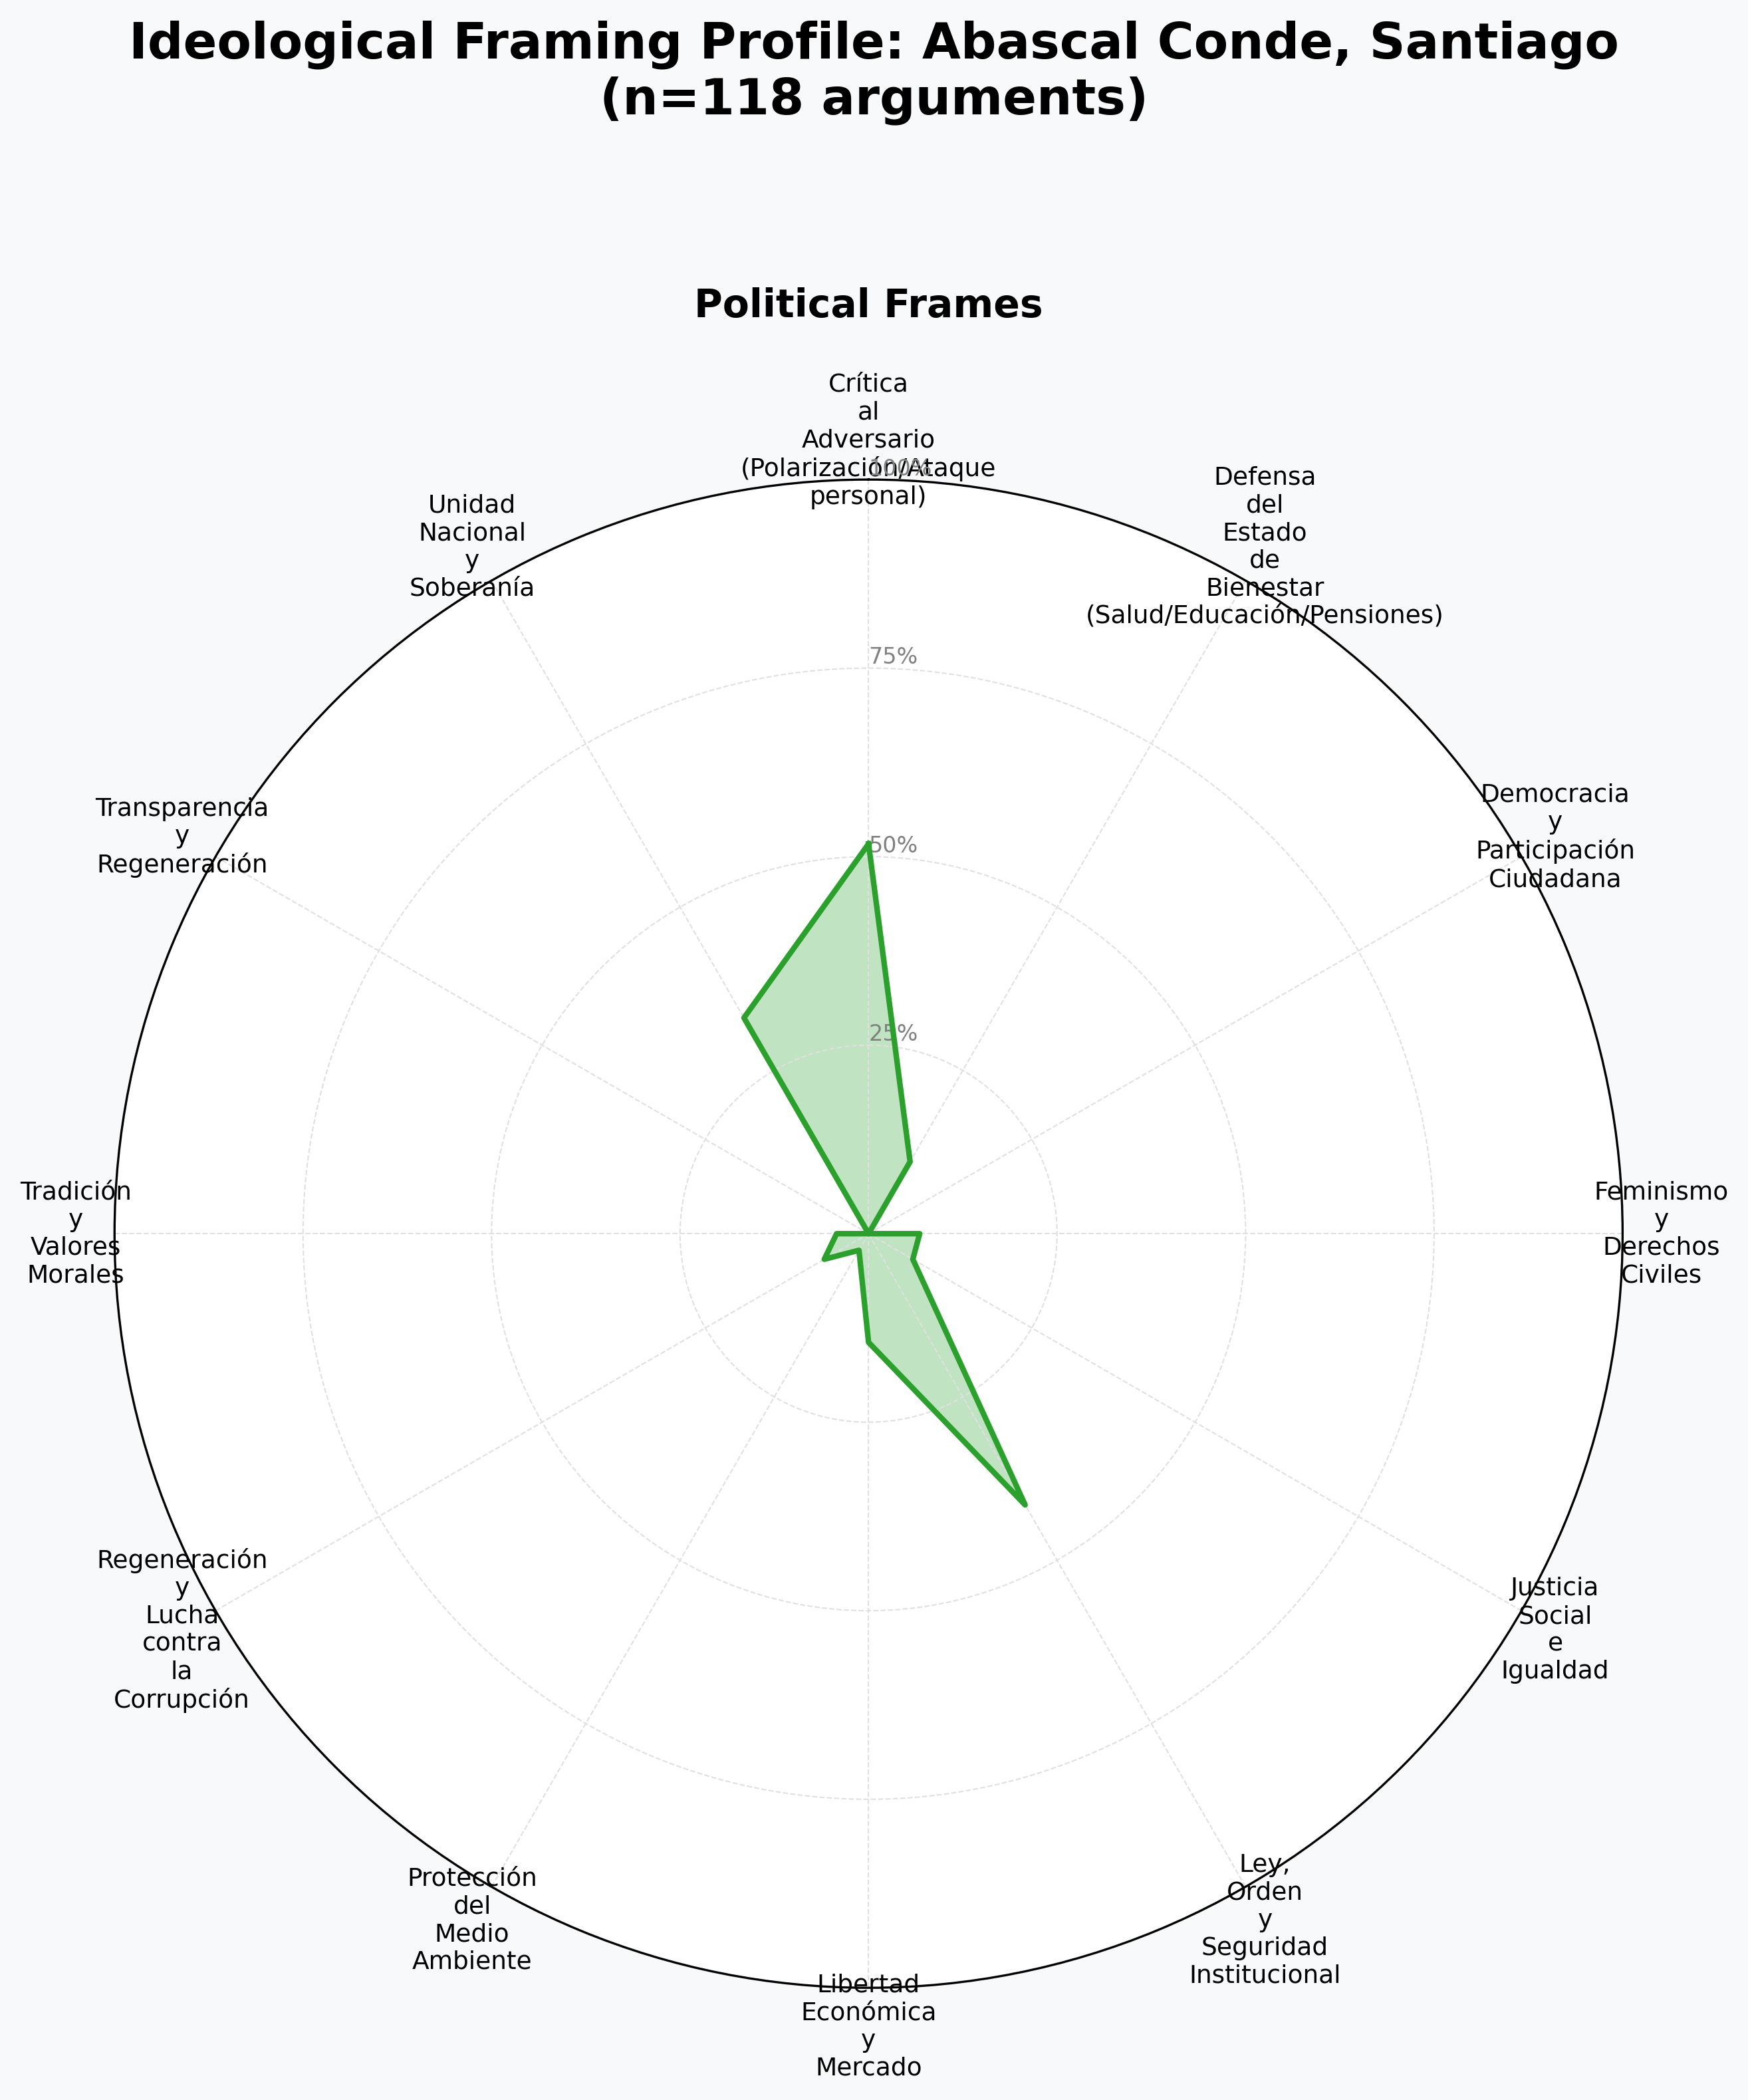
\includegraphics[width=\linewidth]{reports/figures/abascal_conde_santiago_phase_12_radar.png}
        \caption{Santiago Abascal}
    \end{subfigure}
    \hfill
    \begin{subfigure}[b]{0.45\linewidth}
        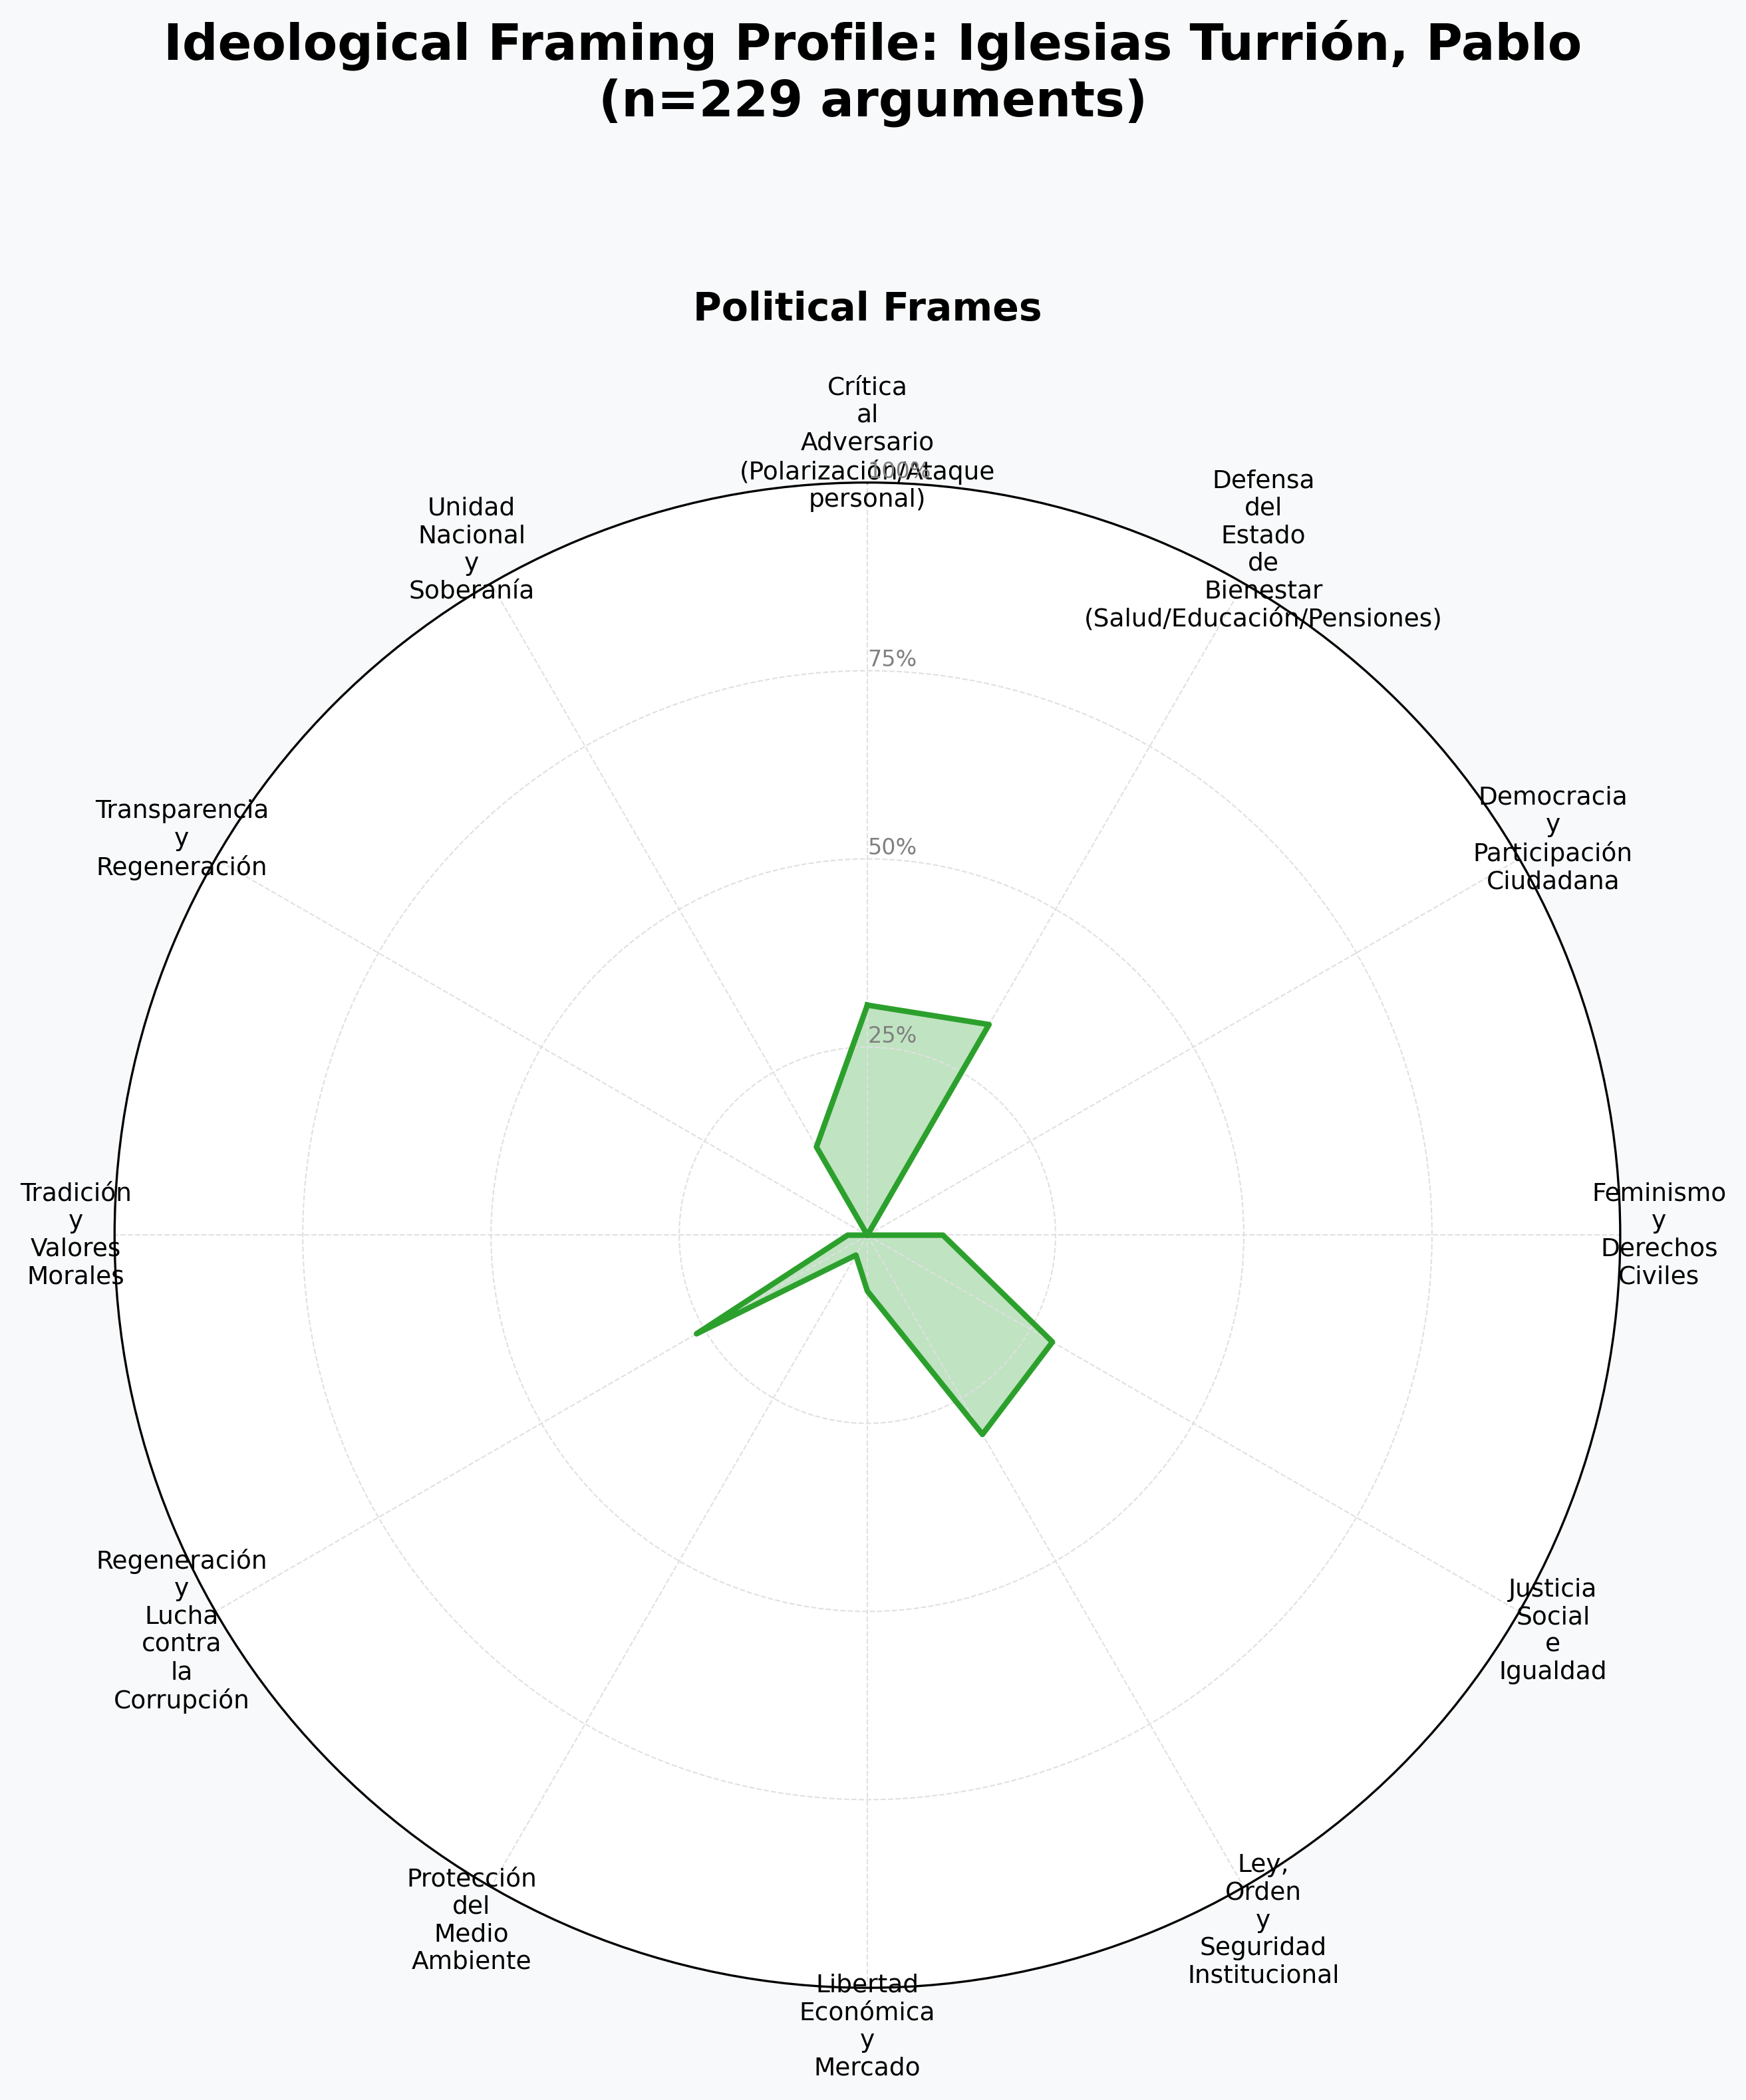
\includegraphics[width=\linewidth]{reports/figures/iglesias_turrión_pablo_phase_12_radar.png}
        \caption{Pablo Iglesias}
    \end{subfigure}
    \\
    \begin{subfigure}[b]{0.45\linewidth}
        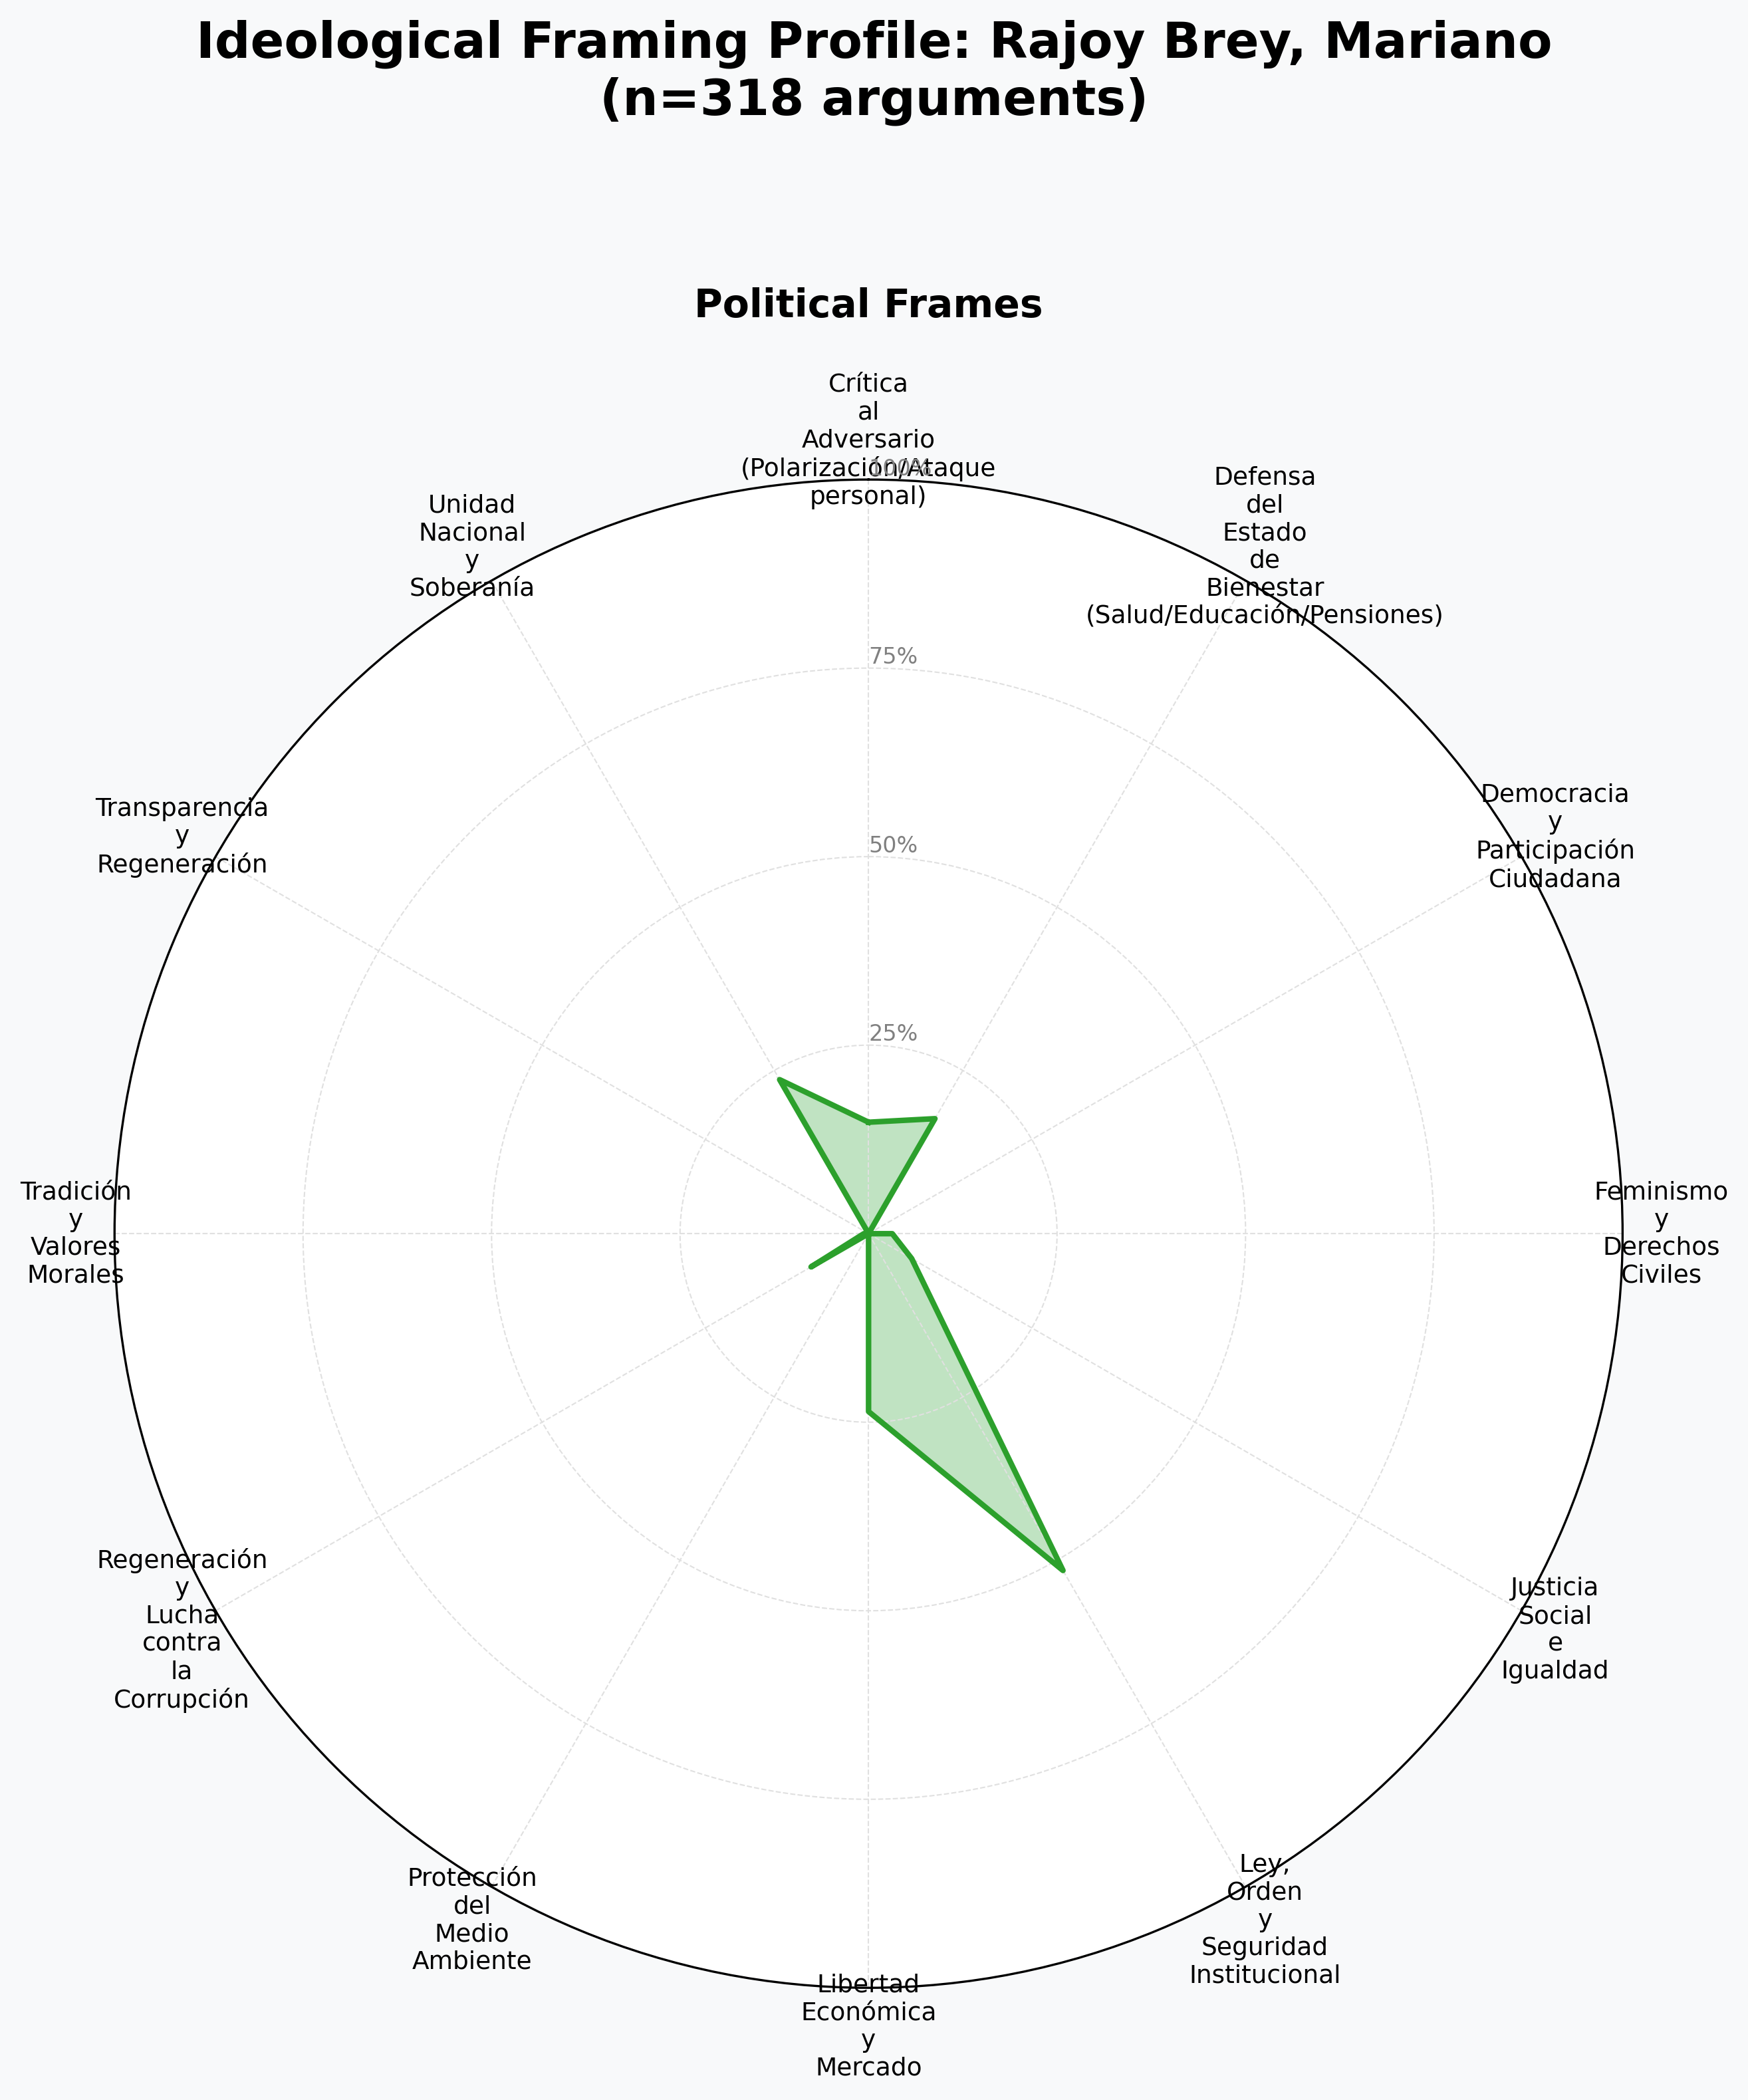
\includegraphics[width=\linewidth]{reports/figures/rajoy_brey_mariano_phase_12_radar.png}
        \caption{Mariano Rajoy}
    \end{subfigure}
    \hfill
    \begin{subfigure}[b]{0.45\linewidth}
        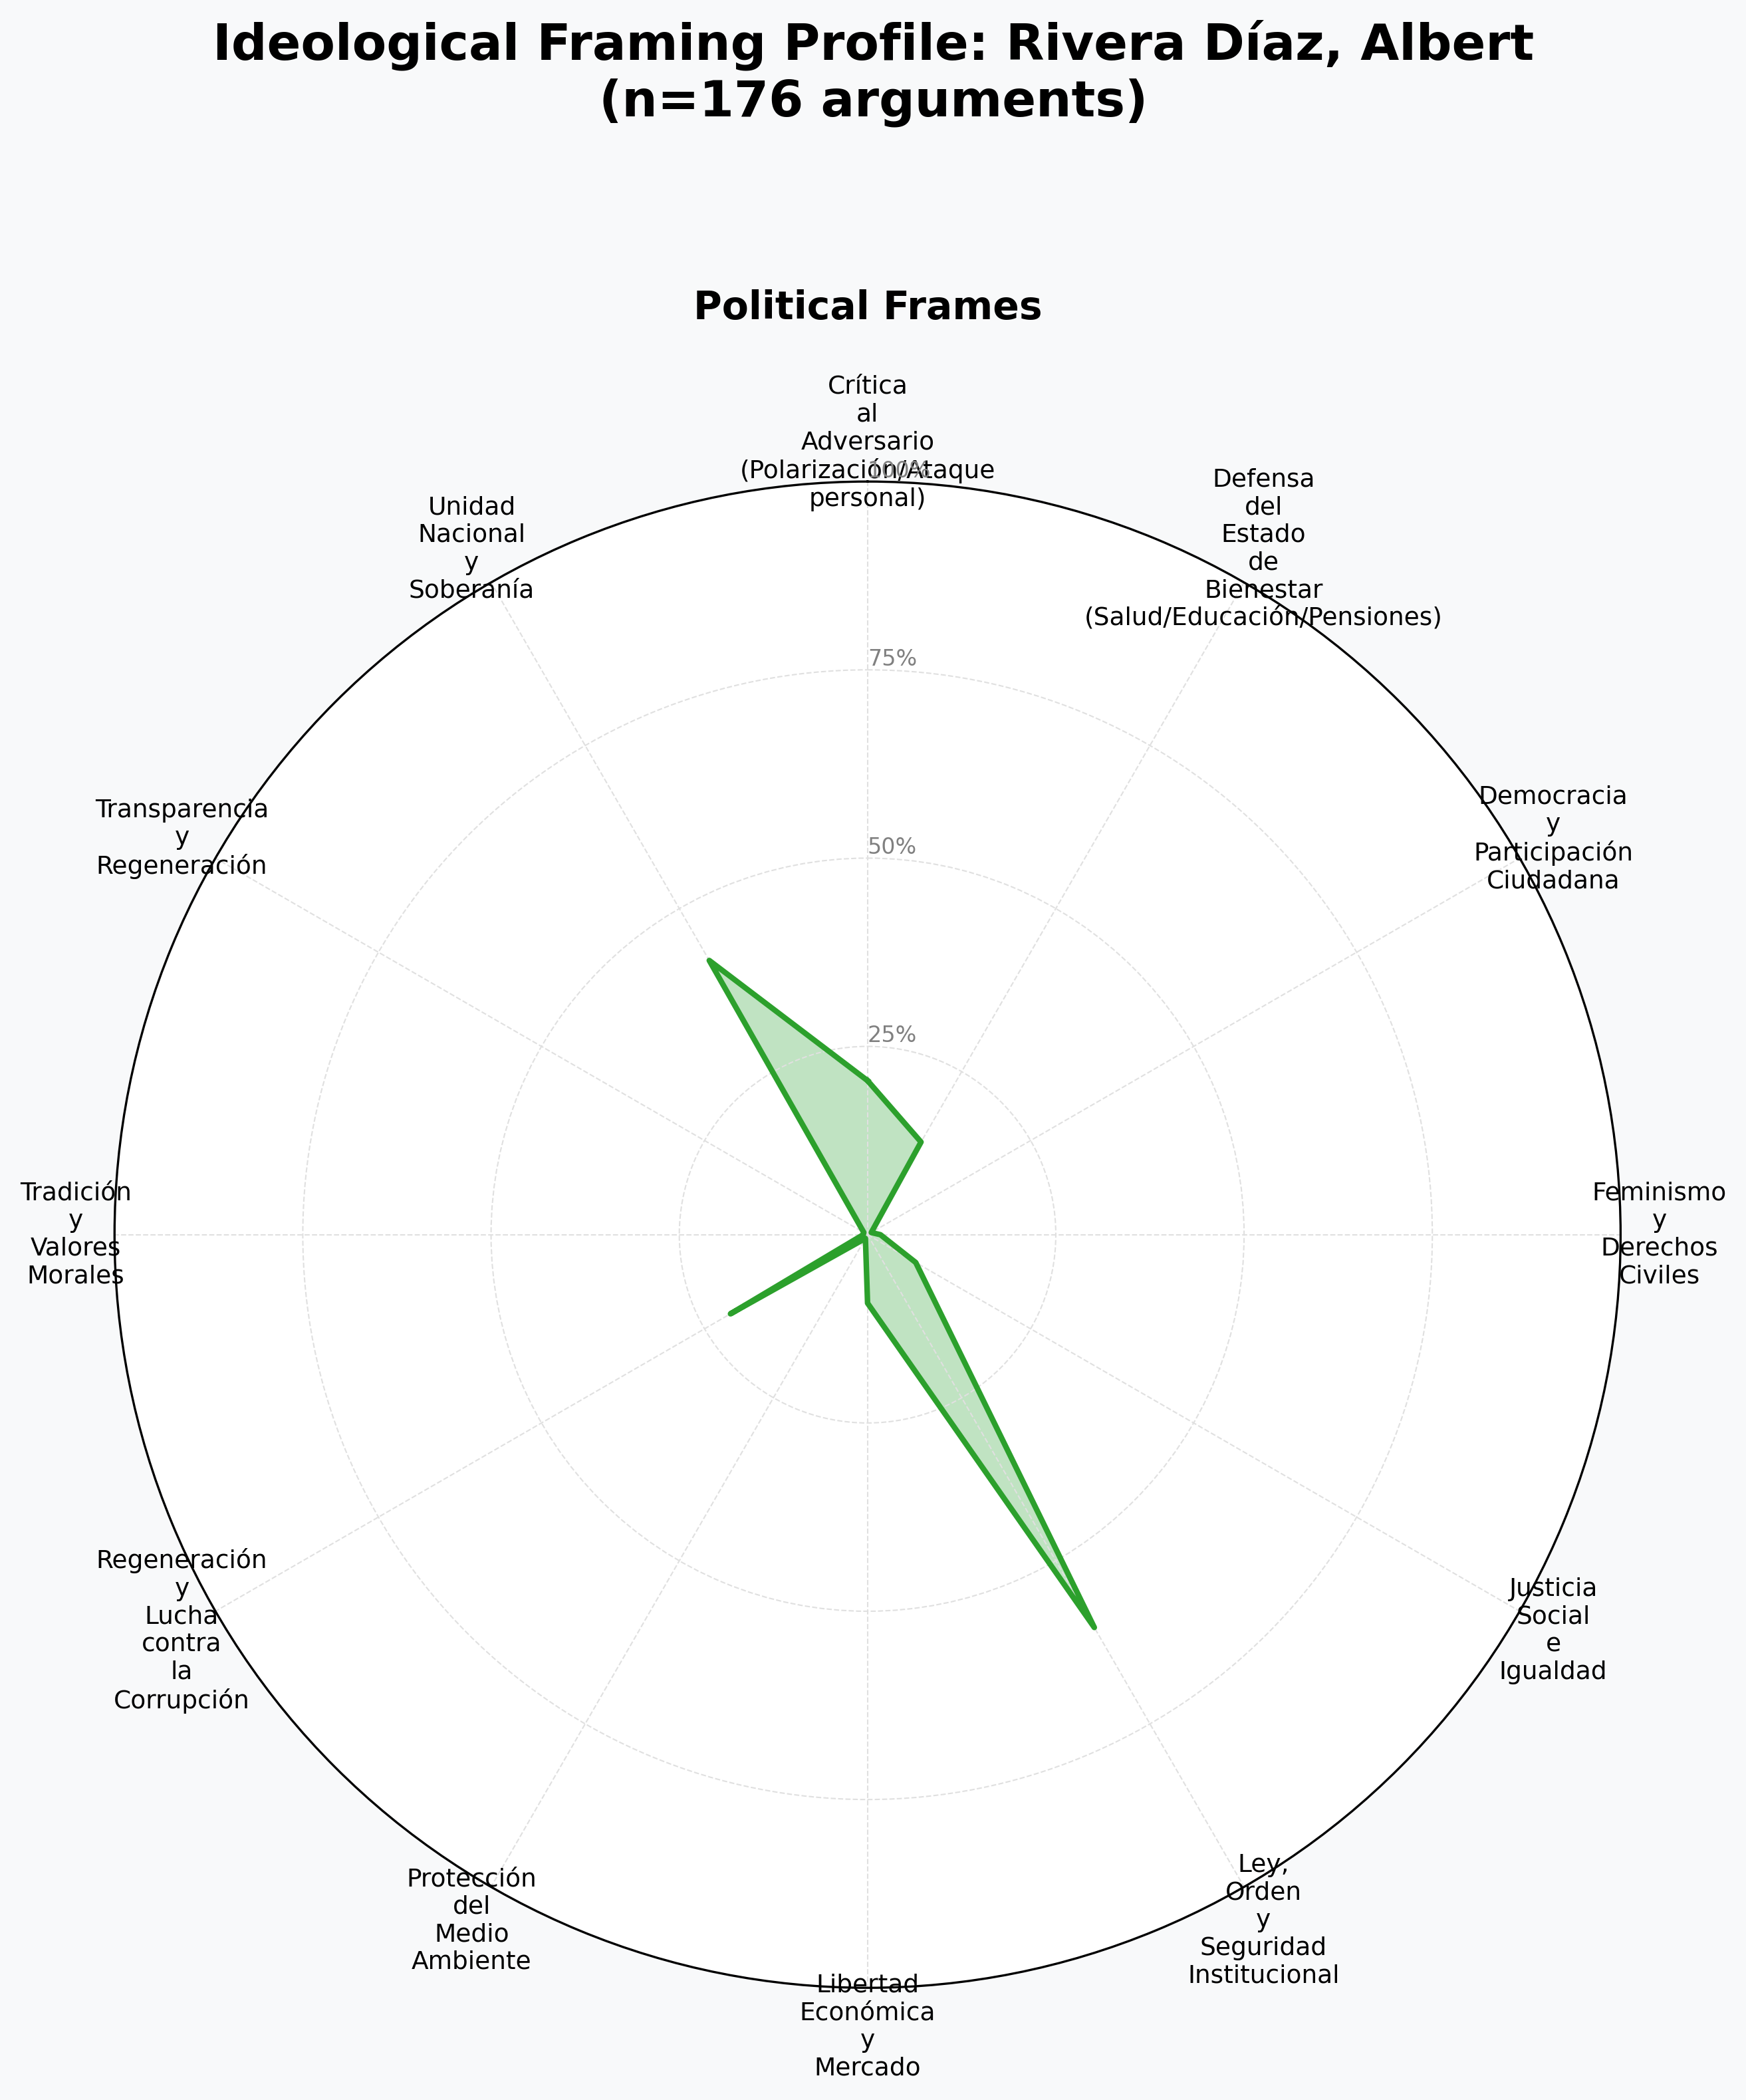
\includegraphics[width=\linewidth]{reports/figures/rivera_díaz_albert_phase_12_radar.png}
        \caption{Albert Rivera}
    \end{subfigure}
    \\
    \begin{subfigure}[b]{0.45\linewidth}
        \centering
        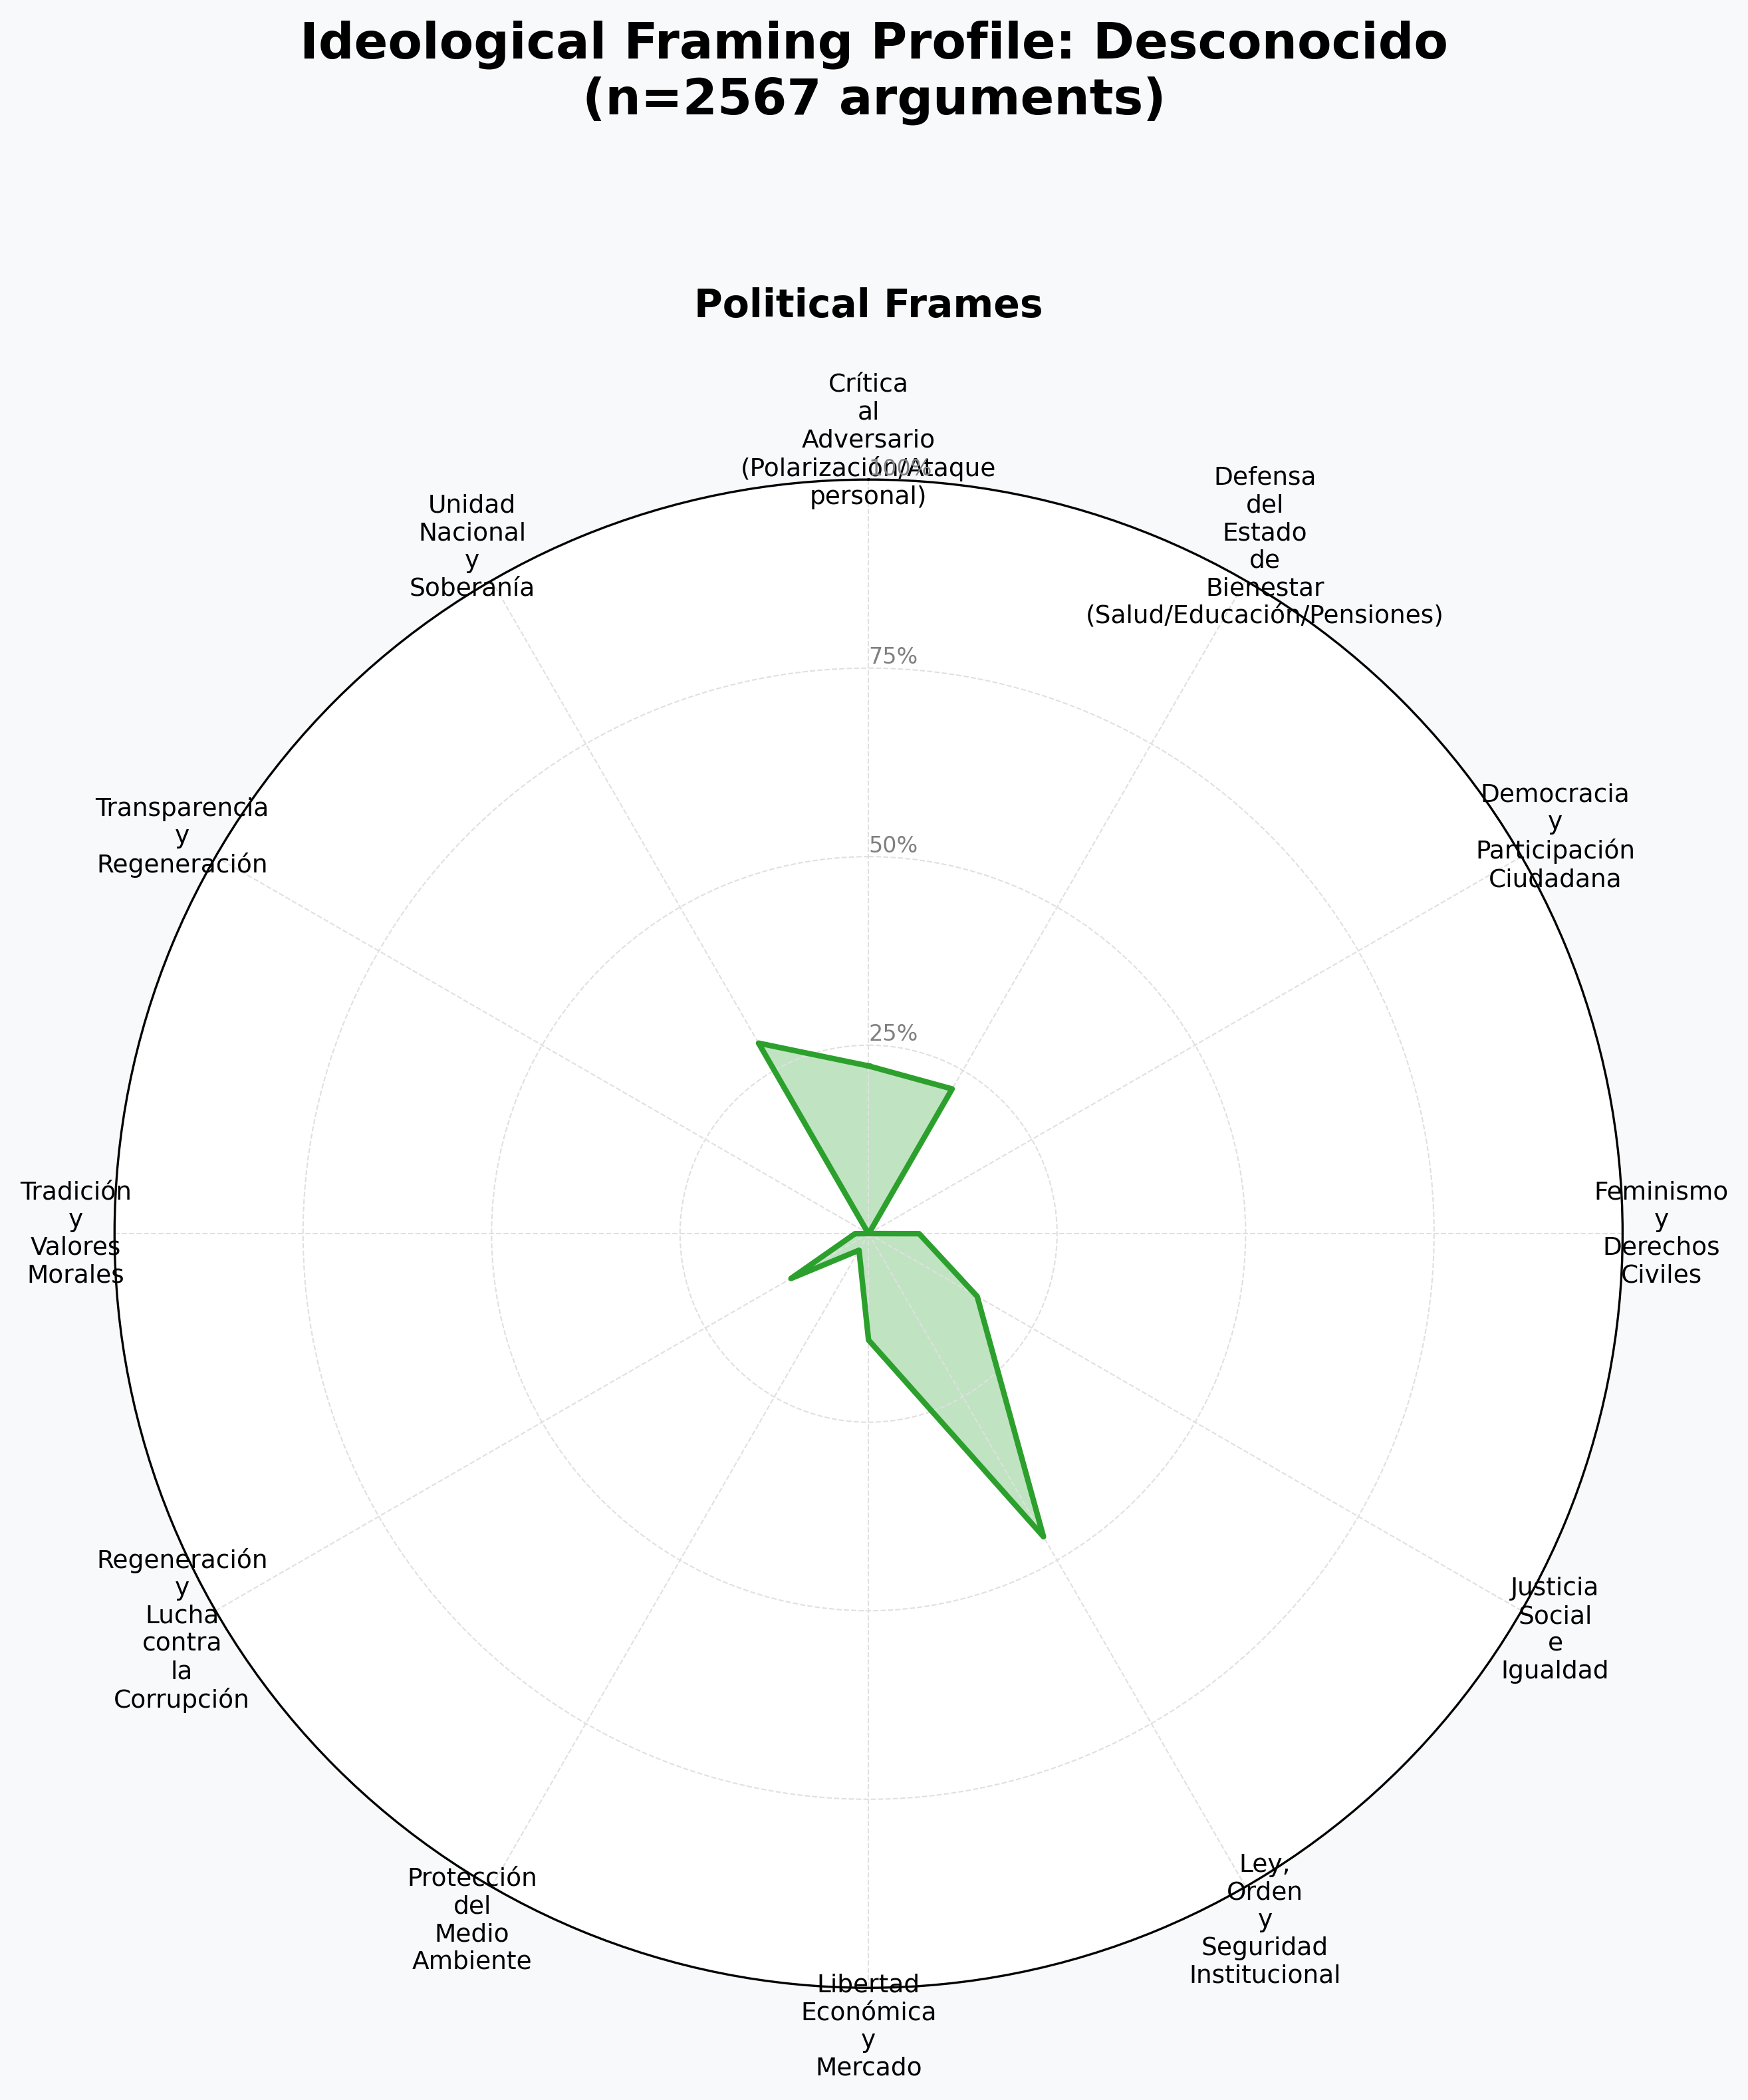
\includegraphics[width=\linewidth]{reports/figures/desconocido_phase_12_radar.png}
        \caption{Desconocido (Parliament Baseline)}
    \end{subfigure}
    \caption{Political Frame Radar Charts across Spanish politicians.}
    \label{fig:radar_charts}
\end{figure}

\subsection{Oppositional Framing and Incumbency}
Beyond individual profiles, we utilized our model to track specific discourse strategies. By ranking politicians based on the frequency of the \textit{Crítica al Adversario} (Attacking the Opponent) frame, we can empirically measure polarization. 

\begin{figure}[htbp]
    \centering
    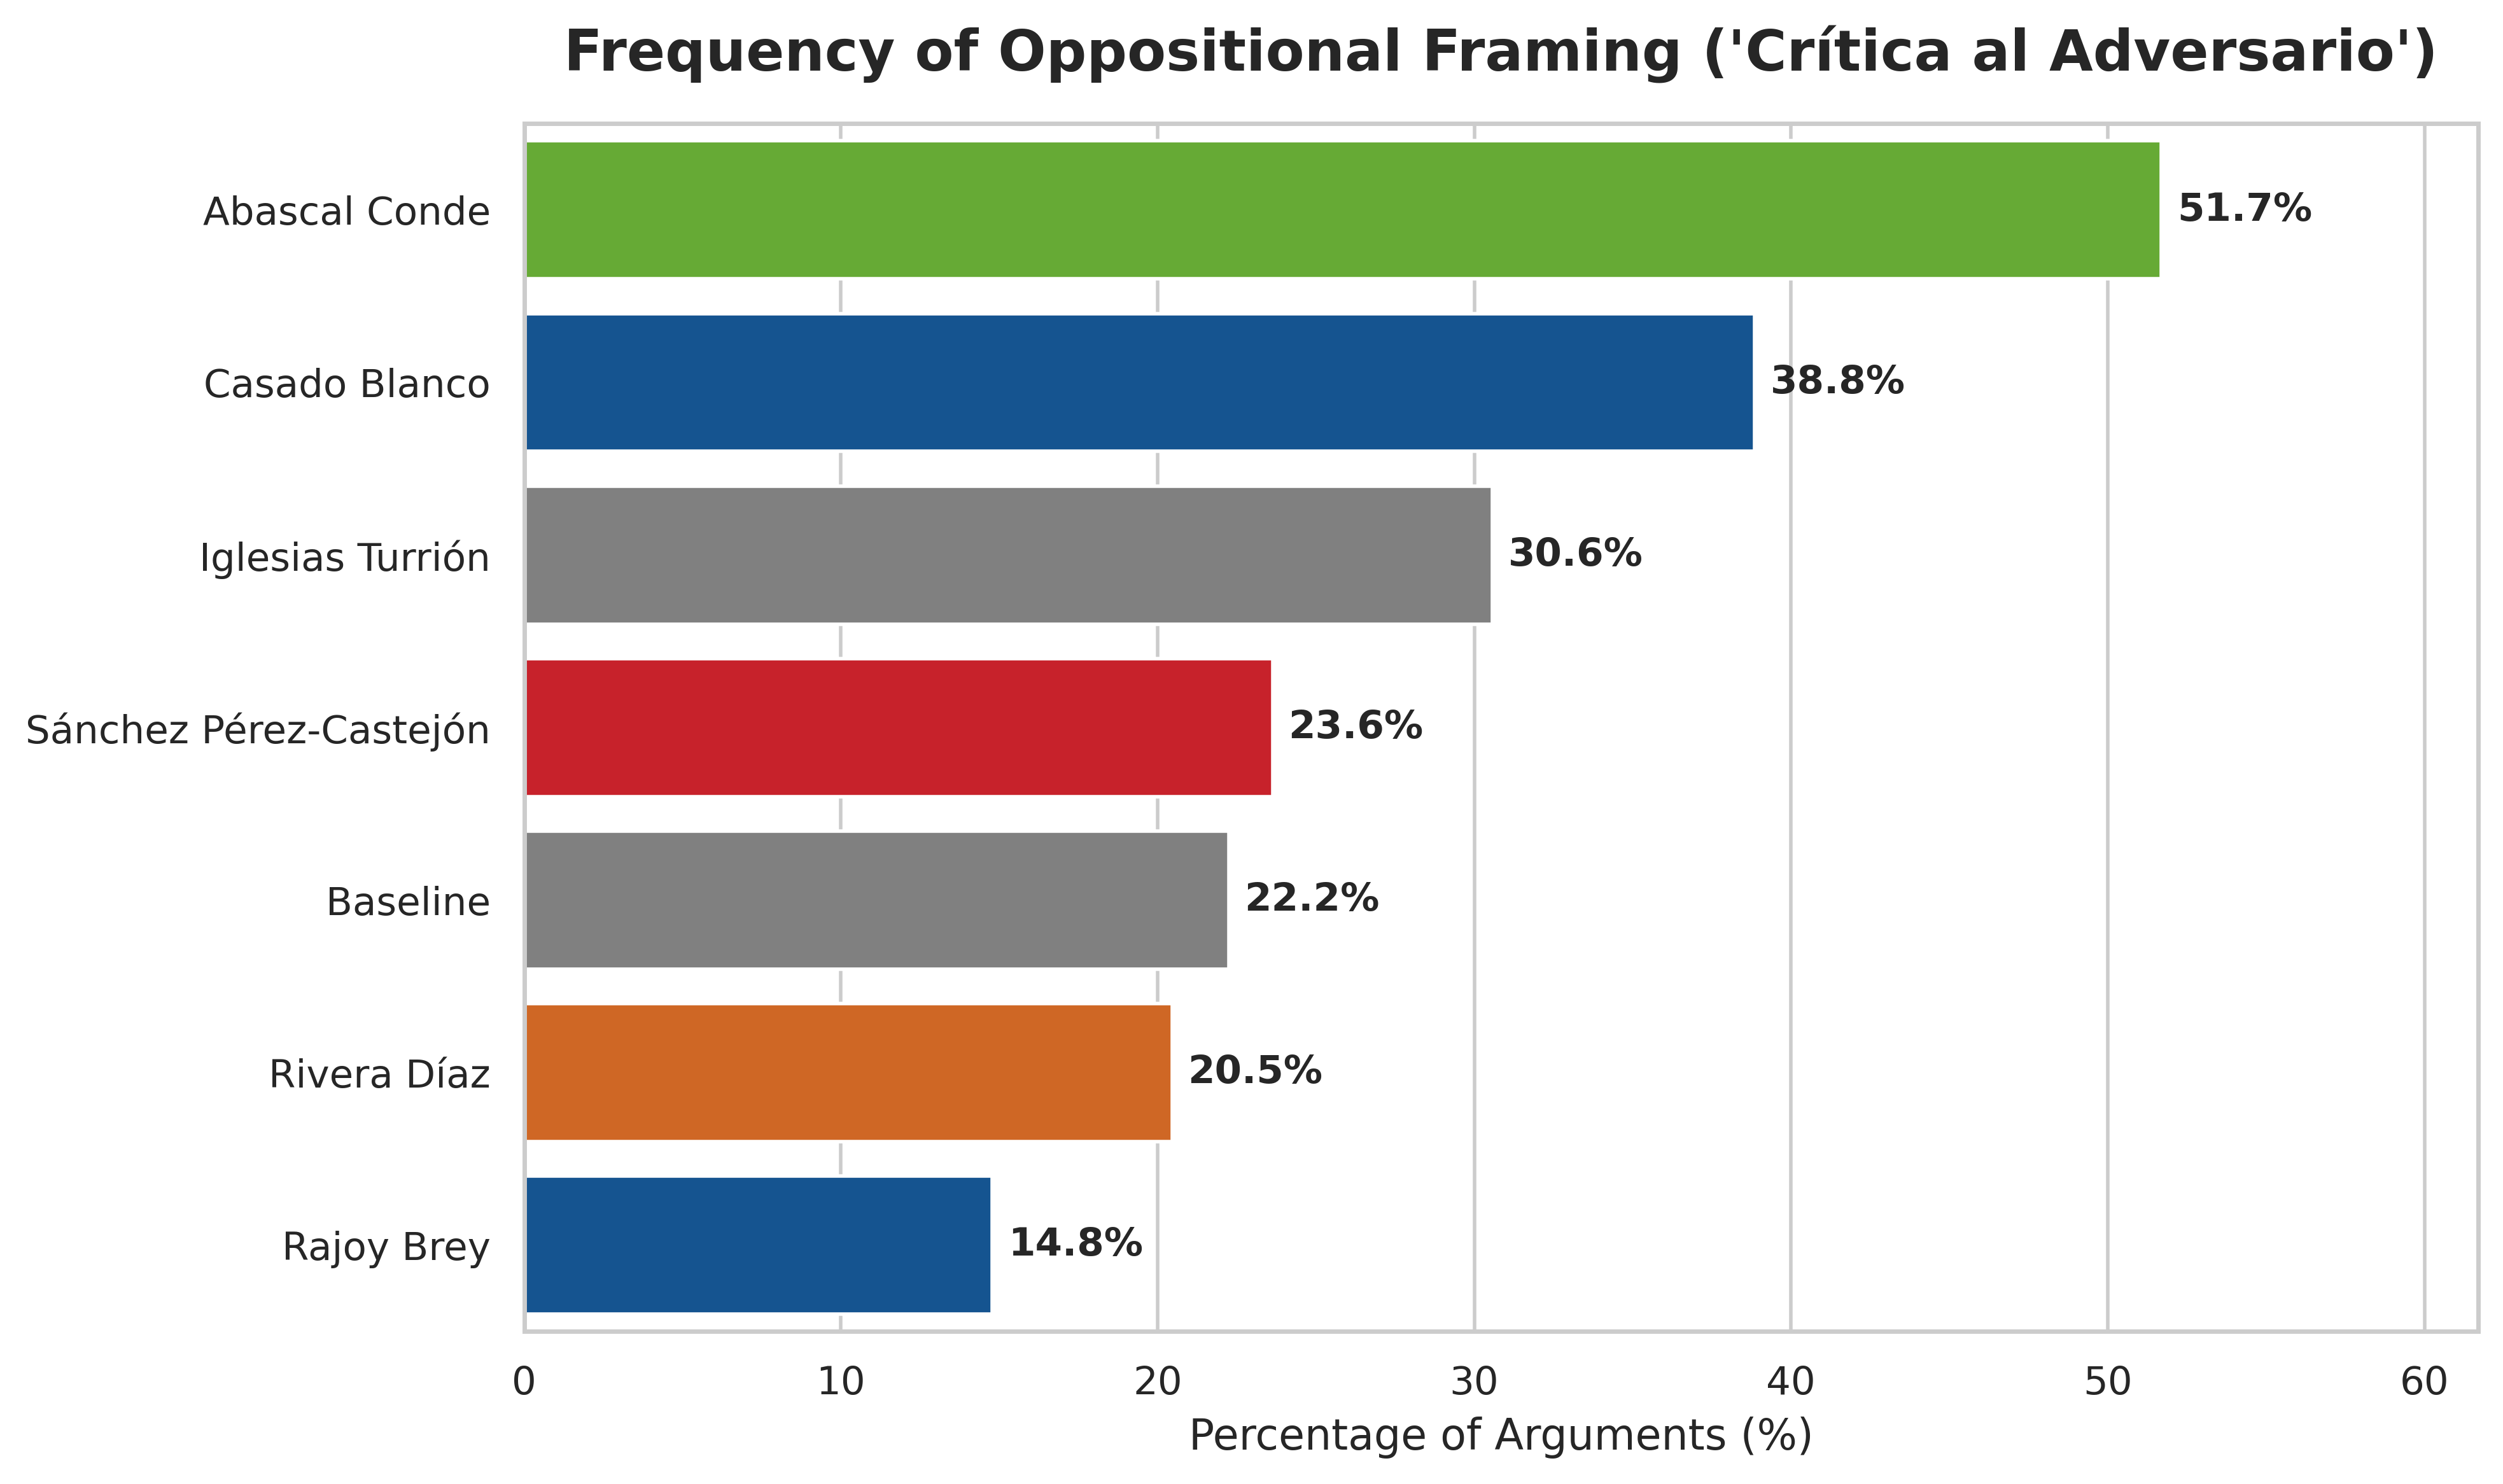
\includegraphics[width=0.9\linewidth]{reports/figures/ranking_critica_adversario.png}
    \caption{Usage percentage of the "Crítica al Adversario" frame by politician compared to the parliamentary baseline.}
    \label{fig:ranking_critica}
\end{figure}

As seen in Figure \ref{fig:ranking_critica}, certain actors significantly outpace the parliamentary baseline in utilizing oppositional framing. However, this metric must be contextualized by incumbency: criticizing the opponent is a primary structural function of the opposition. Consequently, leaders who spent the vast majority of the 2015-2023 period strictly in the opposition (e.g., Santiago Abascal, Pablo Casado, Albert Rivera) naturally index higher on this frame. Conversely, leaders who held executive power during this timeframe (e.g., Pedro Sánchez, Mariano Rajoy) shift their rhetorical distribution toward policy defense and institutional governance, thereby lowering their relative frequency of direct attacks.

\subsection{Rhetorical Ideological Spectrum}
To visualize the broader ideological distribution, we collapsed the high-dimensional framing data into a 1D ideological gradient. By assigning weights to specific frames (e.g., negative weights for social welfare, positive weights for market freedom and national unity), we plotted the selected politicians along a Left-to-Right spectrum.

\begin{figure}[htbp]
    \centering
    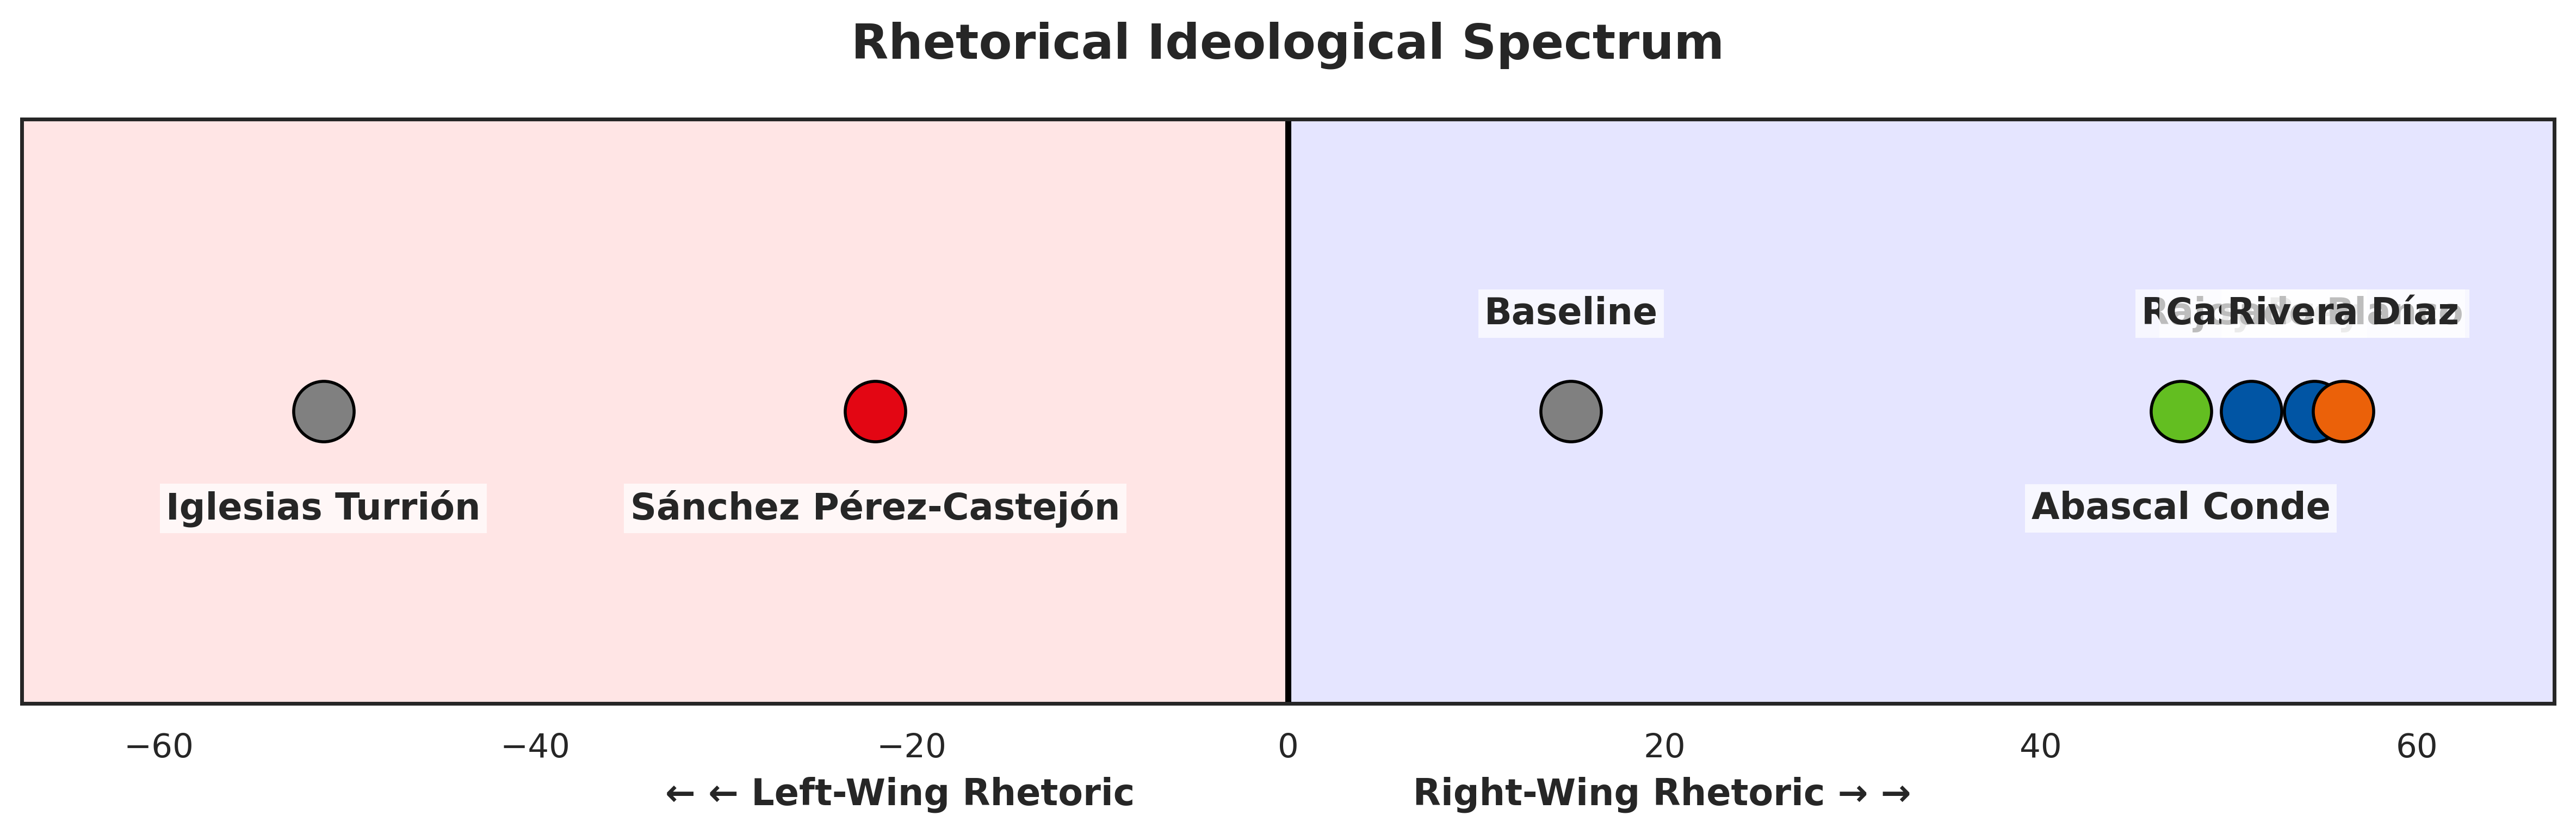
\includegraphics[width=\linewidth]{reports/figures/ideology_gradient.png}
    \caption{Rhetorical Ideological Spectrum (1D Transformation). Values represent the weighted summation of ideological frames.}
    \label{fig:gradient}
\end{figure}

As shown in Figure \ref{fig:gradient}, the model effectively captures the primary axis of Spanish political conflict. Notably, the ``Desconocido'' baseline is positioned slightly to the right of the center. This lean is expected, as the sample of evaluated high-profile candidates includes a higher proportion of right-leaning leaders (PP, Vox, Cs) relative to the left (PSOE, Podemos), influencing the aggregate parliamentary mean.

\section{Critical Analysis \& Limitations}

\subsection{The Populist Paradox: Rhetoric vs. Institutional Reality}
A critical limitation of relying solely on NLP-driven argument mining is the inherent divergence between political rhetoric and legislative reality, a dynamic particularly visible in populist movements. Our analysis places certain figures firmly on the left-wing spectrum, driven by heavy reliance on frames such as \textit{Justicia Social}, \textit{Feminismo}, and \textit{Estado de Bienestar}. 

However, external political science literature frequently characterizes left-wing populism by its combative institutionalism—such as aggressive polarization tactics or proposals to strictly regulate opposing political factions. Our model captures the \textit{emancipatory framing} of their discourse but cannot inherently measure the \textit{authoritarian or restrictive mechanisms} proposed to enforce those social visions. This reveals a 'Populist Paradox' in text analysis: politicians who utilize the highest volume of social-libertarian vocabulary may simultaneously employ highly polarizing, anti-pluralist institutional strategies. 

\subsection{Metadata Brittleness and Error Analysis}
An immediate systematic point of failure occurred during the generation phase with the LLM arbitrarily altering casing for JSON properties. This led to thousands of data points initially losing metadata tags and falling under a ``Desconocido'' label. While our parsing logic corrected this, it underscores the brittleness of querying massive generative LLMs for highly structured output schemas. Furthermore, distinguishing between adjacent economic framing styles occasionally saturated the dynamic class weights, illustrating inherent overlapping ambiguities in the taxonomy.

\subsection{Cost, Latency, and Inherent Bias}
The initial data extraction leveraging a 72B parameter model required massive computational overhead and experienced considerable inference latency unsuited for real-time applications. Concurrently, the deployment of the student RoBERTa classifier radically shifts this paradigm, achieving high-throughput inference manageable on consumer hardware.

However, relying entirely on a zero-shot generative LLM as our initial annotation medium establishes a critical dependency on the inherent alignment biases embedded in the Qwen 72B model. Because the RoBERTa classifier directly learns to mimic the Qwen annotations, it undeniably distills and inherits these precise ideological biases, crystallizing them permanently into its production classifications.

\section{Conclusion}
This study validates a dual-model LLM framework for sophisticated argument mining, combining the heavy extraction capabilities of a 72B Instruct model with the speed and deployment efficiency of a distilled RoBERTa text classifier, successfully mapping ideological frames and rhetorical strategies within Spanish political discourse.

\end{document}